\documentclass[10pt,a4paper]{article}
\usepackage[margin=2cm]{geometry}
\usepackage[T1]{fontenc}
\usepackage{amsmath,amssymb,booktabs,longtable,graphicx,float}
\usepackage[hyphens]{url}
\usepackage[hidelinks]{hyperref}
\graphicspath{{figures/}}
\newcommand{\aperp}{\alpha_{\perp}}
\renewcommand{\thetable}{S\arabic{table}}
\renewcommand{\thefigure}{S\arabic{figure}}
\title{Supplementary Material:\\ Portfolio-Conditioned Dynamic Weakness and Reinforcement Ranking in Inverter-Rich Power Networks}
\author{Jorge L.~Mayorga Taborda}
\date{}
\begin{document}
\maketitle
\section{Policy holdout}
The new holdout HARDENING\_H01--H24 (N01--N24) is the maximin Latin hypercube of 2000 candidates (seed 20260929; minimum pairwise distance 0.3233 in the unit cube). The file \path{results/hardening/prereg_inputs/hardening_policies.json} has sha256 \texttt{53640af64825587f\ldots}.

{\scriptsize
\begin{longtable}{lcccccc}
\caption{New holdout policies ($g=u^2$).}\label{tab:s-pol}\\
\toprule
id & $g$ & $k$ & $t$ & $h$ & $\aperp(\emptyset)$ & base \\
\midrule
\endfirsthead
\toprule
id & $g$ & $k$ & $t$ & $h$ & $\aperp(\emptyset)$ & base \\
\midrule
\endhead
N01 & 0.9921 & 1.264 & 2.732 & 1.130 & -0.150 & stable \\
N02 & 0.9036 & 2.174 & 0.650 & 0.703 & 0.222 & unstable \\
N03 & 0.4711 & 1.376 & 2.531 & 1.402 & -0.153 & stable \\
N04 & 0.1473 & 0.701 & 1.572 & 0.896 & -0.172 & stable \\
N05 & 0.6857 & 0.764 & 2.359 & 1.509 & -0.170 & stable \\
N06 & 0.8025 & 0.851 & 0.991 & 0.540 & -0.125 & stable \\
N07 & 0.7573 & 1.979 & 1.717 & 0.082 & 0.005 & unstable \\
N08 & 0.0628 & 2.278 & 1.496 & 1.000 & 0.022 & unstable \\
N09 & 0.0276 & 1.222 & 2.104 & 0.640 & -0.167 & stable \\
N10 & 0.2312 & 0.877 & 1.919 & 1.861 & -0.176 & stable \\
N11 & 0.0001 & 1.548 & 1.384 & 0.251 & -0.042 & stable \\
N12 & 0.1812 & 1.023 & 0.862 & 1.239 & -0.109 & stable \\
N13 & 0.0338 & 0.598 & 2.471 & 0.408 & -0.179 & stable \\
N14 & 0.0066 & 1.025 & 2.914 & 0.219 & -0.174 & stable \\
N15 & 0.0129 & 1.827 & 0.792 & 1.597 & 0.115 & unstable \\
N16 & 0.3887 & 1.893 & 1.753 & 0.488 & -0.098 & stable \\
N17 & 0.2655 & 1.681 & 1.301 & 1.808 & -0.129 & stable \\
N18 & 0.1087 & 1.583 & 1.977 & 1.474 & -0.165 & stable \\
N19 & 0.6048 & 2.073 & 2.854 & 1.709 & -0.126 & stable \\
N20 & 0.4438 & 1.142 & 1.121 & 1.952 & -0.149 & stable \\
N21 & 0.2994 & 0.560 & 2.592 & 0.116 & -0.178 & stable \\
N22 & 0.1228 & 1.759 & 2.200 & 0.818 & -0.160 & stable \\
N23 & 0.5486 & 2.102 & 0.599 & 1.317 & 0.136 & unstable \\
N24 & 0.0579 & 1.456 & 1.164 & 0.961 & -0.084 & stable \\
\bottomrule
\end{longtable}}


\section{Per-policy census summary}
Columns rev./A/B/C: number of units (of nine) with a stable-context reversal (any pair) or a nested reversal at levels A/B/C. The full marginal table (2304 marginals per policy, 63 policies) is \path{results/hardening/H03_marginals.parquet}; all nested pairs with their curvature witnesses are in \path{H03_nested_pairs.parquet}.

{\tiny
\begin{longtable}{lllrrrrrrrrr}
\caption{Per-policy reversal counts and oracle fixed-ranking results (FULL stratum).}\label{tab:s-census}\\
\toprule
policy & set & stable base & rev. & A & B & C & C pairs & C s$\to$d/d$\to$s & C max mag & $p^\star$ & regret \\
\midrule
\endfirsthead
\toprule
policy & set & stable base & rev. & A & B & C & C pairs & C s$\to$d/d$\to$s & C max mag & $p^\star$ & regret \\
\midrule
\endhead
D01 & discovery & y & 9 & 9 & 8 & 8 & 145 & 143/2 & 0.045 & 0.667 & 0.483 \\
D02 & discovery & y & 8 & 8 & 4 & 4 & 65 & 0/65 & 0.017 & 0.722 & 0.403 \\
D03 & discovery & y & 8 & 8 & 7 & 7 & 383 & 0/383 & 0.036 & 0.811 & 0.351 \\
D04 & discovery & y & 1 & 1 & 0 & 0 & 0 & 0/0 & -- & 0.768 & 0.164 \\
D05 & discovery & y & 8 & 8 & 7 & 7 & 265 & 204/61 & 0.041 & 0.794 & 0.384 \\
D06 & discovery & y & 8 & 8 & 7 & 7 & 420 & 0/420 & 0.031 & 0.786 & 0.383 \\
D07 & discovery & y & 8 & 8 & 7 & 7 & 309 & 0/309 & 0.031 & 0.766 & 0.348 \\
D08 & discovery & y & 8 & 8 & 6 & 6 & 512 & 511/1 & 0.037 & 0.686 & 0.444 \\
D09 & discovery & y & 8 & 8 & 7 & 7 & 491 & 0/491 & 0.031 & 0.801 & 0.384 \\
D10 & discovery & y & 9 & 9 & 6 & 6 & 161 & 73/88 & 0.029 & 0.795 & 0.360 \\
D11 & discovery & y & 8 & 8 & 5 & 5 & 120 & 1/119 & 0.036 & 0.827 & 0.345 \\
D12 & discovery & y & 8 & 8 & 6 & 6 & 162 & 12/150 & 0.031 & 0.797 & 0.381 \\
D13 & discovery & y & 8 & 8 & 2 & 2 & 66 & 0/66 & 0.016 & 0.759 & 0.355 \\
D14 & discovery & y & 7 & 7 & 4 & 4 & 134 & 0/134 & 0.038 & 0.824 & 0.336 \\
D15 & discovery & y & 8 & 8 & 6 & 6 & 206 & 0/206 & 0.031 & 0.775 & 0.356 \\
H01 & old & n & 6 & 6 & 1 & 1 & 3 & 0/3 & 0.029 & 0.726 & 0.435 \\
H02 & old & y & 9 & 9 & 6 & 4 & 5 & 5/0 & 0.022 & 0.638 & 0.388 \\
H03 & old & n & 4 & 4 & 1 & 0 & 0 & 0/0 & -- & 0.643 & 0.458 \\
H04 & old & y & 9 & 9 & 2 & 2 & 48 & 6/42 & 0.025 & 0.753 & 0.380 \\
H05 & old & y & 1 & 1 & 0 & 0 & 0 & 0/0 & -- & 0.841 & 0.152 \\
H06 & old & n & 7 & 7 & 5 & 5 & 56 & 0/56 & 0.020 & 0.760 & 0.304 \\
H07 & old & y & 8 & 8 & 6 & 6 & 193 & 0/193 & 0.030 & 0.783 & 0.380 \\
H08 & old & y & 8 & 8 & 2 & 2 & 60 & 0/60 & 0.017 & 0.757 & 0.366 \\
H09 & old & y & 9 & 9 & 2 & 2 & 39 & 0/39 & 0.016 & 0.722 & 0.402 \\
H10 & old & y & 8 & 8 & 7 & 7 & 254 & 0/254 & 0.030 & 0.750 & 0.358 \\
H11 & old & y & 9 & 9 & 5 & 5 & 61 & 0/61 & 0.018 & 0.734 & 0.358 \\
H12 & old & y & 9 & 9 & 7 & 7 & 129 & 128/1 & 0.040 & 0.666 & 0.425 \\
H13 & old & y & 1 & 1 & 0 & 0 & 0 & 0/0 & -- & 0.733 & 0.229 \\
H14 & old & y & 8 & 8 & 5 & 5 & 174 & 0/174 & 0.019 & 0.784 & 0.350 \\
H15 & old & y & 8 & 8 & 7 & 7 & 294 & 250/44 & 0.040 & 0.815 & 0.310 \\
H16 & old & n & 5 & 5 & 0 & 0 & 0 & 0/0 & -- & 0.677 & 0.524 \\
H17 & old & n & 7 & 7 & 1 & 1 & 4 & 0/4 & 0.013 & 0.725 & 0.375 \\
H18 & old & y & 8 & 8 & 7 & 7 & 412 & 0/412 & 0.027 & 0.769 & 0.372 \\
H19 & old & y & 8 & 8 & 5 & 5 & 290 & 0/290 & 0.038 & 0.820 & 0.336 \\
H20 & old & n & 7 & 7 & 4 & 4 & 103 & 0/103 & 0.033 & 0.764 & 0.320 \\
H21 & old & y & 8 & 8 & 3 & 3 & 45 & 0/45 & 0.017 & 0.734 & 0.405 \\
H22 & old & y & 8 & 8 & 7 & 7 & 605 & 0/605 & 0.032 & 0.808 & 0.352 \\
H23 & old & y & 8 & 8 & 6 & 6 & 438 & 429/9 & 0.035 & 0.695 & 0.442 \\
H24 & old & y & 8 & 8 & 8 & 8 & 452 & 408/44 & 0.047 & 0.734 & 0.397 \\
N01 & new & y & 9 & 9 & 4 & 4 & 66 & 0/66 & 0.016 & 0.725 & 0.412 \\
N02 & new & n & 6 & 6 & 0 & 0 & 0 & 0/0 & -- & 0.726 & 0.452 \\
N03 & new & y & 9 & 9 & 5 & 5 & 98 & 0/98 & 0.021 & 0.757 & 0.353 \\
N04 & new & y & 8 & 8 & 4 & 4 & 245 & 244/1 & 0.030 & 0.740 & 0.380 \\
N05 & new & y & 8 & 8 & 2 & 2 & 39 & 0/39 & 0.015 & 0.725 & 0.410 \\
N06 & new & y & 8 & 8 & 5 & 5 & 162 & 0/162 & 0.031 & 0.771 & 0.363 \\
N07 & new & n & 8 & 8 & 6 & 6 & 136 & 0/136 & 0.032 & 0.756 & 0.305 \\
N08 & new & n & 8 & 8 & 5 & 5 & 59 & 13/46 & 0.068 & 0.824 & 0.287 \\
N09 & new & y & 9 & 9 & 9 & 7 & 50 & 50/0 & 0.040 & 0.622 & 0.422 \\
N10 & new & y & 8 & 8 & 3 & 3 & 14 & 12/2 & 0.027 & 0.747 & 0.379 \\
N11 & new & y & 3 & 3 & 0 & 0 & 0 & 0/0 & -- & 0.775 & 0.167 \\
N12 & new & y & 7 & 7 & 4 & 4 & 103 & 1/102 & 0.032 & 0.825 & 0.376 \\
N13 & new & y & 9 & 9 & 8 & 7 & 87 & 87/0 & 0.037 & 0.654 & 0.442 \\
N14 & new & y & 2 & 2 & 1 & 0 & 0 & 0/0 & -- & 0.749 & 0.268 \\
N15 & new & n & 6 & 6 & 3 & 1 & 1 & 1/0 & 0.028 & 0.698 & 0.518 \\
N16 & new & y & 8 & 8 & 7 & 7 & 505 & 0/505 & 0.030 & 0.810 & 0.340 \\
N17 & new & y & 7 & 7 & 6 & 6 & 500 & 0/500 & 0.036 & 0.814 & 0.387 \\
N18 & new & y & 8 & 8 & 7 & 7 & 477 & 474/3 & 0.031 & 0.733 & 0.417 \\
N19 & new & y & 9 & 9 & 6 & 6 & 142 & 0/142 & 0.022 & 0.747 & 0.360 \\
N20 & new & y & 8 & 8 & 6 & 6 & 208 & 0/208 & 0.030 & 0.786 & 0.368 \\
N21 & new & y & 8 & 8 & 2 & 2 & 14 & 7/7 & 0.025 & 0.745 & 0.375 \\
N22 & new & y & 8 & 8 & 5 & 5 & 239 & 124/115 & 0.040 & 0.783 & 0.380 \\
N23 & new & n & 6 & 5 & 0 & 0 & 0 & 0/0 & -- & 0.723 & 0.595 \\
N24 & new & y & 8 & 8 & 7 & 7 & 118 & 78/40 & 0.042 & 0.832 & 0.325 \\
\bottomrule
\end{longtable}}


\section{Minimal curvature witnesses}
For each new-holdout policy and direction, the level-C nested reversal with the smallest chain length (or, if none has $m=1$, the largest magnitude), and the certifying second difference $d_{ij}$ on the canonical chain (Proposition~2 of the paper). s$\to$d needs $d>0$ (a submodularity violation), d$\to$s needs $d<0$ (a supermodularity violation).

{\tiny
\begin{longtable}{llcllrrcrc}
\caption{Minimal nested EM same-mode reversals and certifying curvature terms (s$^{-1}$).}\label{tab:s-wit}\\
\toprule
policy & dir & $i$ & $S_1$ & $S_2$ & $\Delta(S_1)$ & $\Delta(S_2)$ & $j$ & $d_{ij}$ & EM-clean \\
\midrule
\endfirsthead
\toprule
policy & dir & $i$ & $S_1$ & $S_2$ & $\Delta(S_1)$ & $\Delta(S_2)$ & $j$ & $d_{ij}$ & EM-clean \\
\midrule
\endhead
N01 & d$\to$s & 33 & 38 & 34,38 & 0.015 & -0.012 & 34 & -0.027 & y \\
N03 & d$\to$s & 33 & 38 & 34,38 & 0.021 & -0.011 & 34 & -0.032 & y \\
N04 & s$\to$d & 33 & 31,34,38 & 31,34,37,38 & -0.021 & 0.051 & 37 & 0.073 & y \\
N04 & d$\to$s & 34 & 35,37,38 & 30,35,37,38 & 0.030 & -0.036 & 30 & -0.066 & y \\
N05 & d$\to$s & 33 & 38 & 34,38 & 0.012 & -0.012 & 34 & -0.025 & y \\
N06 & d$\to$s & 33 & 38 & 34,38 & 0.022 & -0.012 & 34 & -0.033 & y \\
N07 & d$\to$s & 30 & 32,34,36 & 32,34,36,38 & 0.017 & -0.014 & 38 & -0.031 & y \\
N08 & s$\to$d & 30 & 32,34,38 & 32,34,37,38 & -0.013 & 0.038 & 37 & 0.051 & y \\
N08 & d$\to$s & 30 & 32,34 & 32,34,38 & 0.035 & -0.013 & 38 & -0.048 & y \\
N09 & s$\to$d & 32 & 30,33,35 & 30,33,35,37 & -0.023 & 0.073 & 37 & 0.096 & y \\
N10 & s$\to$d & 34 & 31,35,38 & 31,35,37,38 & -0.024 & 0.031 & 37 & 0.055 & y \\
N10 & d$\to$s & 33 & 35,38 & 34,35,38 & 0.012 & -0.011 & 34 & -0.023 & y \\
N12 & s$\to$d & 31 & 34,35,38 & 34,35,37,38 & -0.012 & 0.012 & 37 & 0.025 & y \\
N12 & d$\to$s & 33 & 31,38 & 31,34,38 & 0.038 & -0.011 & 34 & -0.049 & y \\
N13 & s$\to$d & 34 & 37,38 & 33,37,38 & -0.012 & 0.015 & 33 & 0.027 & y \\
N15 & s$\to$d & 33 & 34,38 & 30,34,38 & -0.028 & 0.039 & 30 & 0.067 & y \\
N16 & d$\to$s & 30 & 32,34,36 & 32,34,36,38 & 0.020 & -0.012 & 38 & -0.032 & y \\
N17 & d$\to$s & 32 & 30,37 & 30,33,37 & 0.011 & -0.012 & 33 & -0.023 & y \\
N18 & s$\to$d & 30 & 31,35 & 31,33,35 & -0.011 & 0.039 & 33 & 0.050 & y \\
N18 & d$\to$s & 34 & 35,37,38 & 30,35,37,38 & 0.030 & -0.053 & 30 & -0.083 & y \\
N19 & d$\to$s & 33 & 38 & 34,38 & 0.027 & -0.011 & 34 & -0.038 & y \\
N20 & d$\to$s & 33 & 38 & 34,38 & 0.029 & -0.011 & 34 & -0.040 & y \\
N21 & s$\to$d & 34 & 31,35,38 & 31,35,37,38 & -0.023 & 0.029 & 37 & 0.051 & y \\
N21 & d$\to$s & 33 & 30,38 & 30,34,38 & 0.012 & -0.012 & 34 & -0.024 & y \\
N22 & s$\to$d & 33 & 31,34,38 & 31,34,37,38 & -0.020 & 0.056 & 37 & 0.076 & y \\
N22 & d$\to$s & 33 & 31,38 & 31,34,38 & 0.013 & -0.020 & 34 & -0.033 & y \\
N24 & s$\to$d & 30 & 36,38 & 33,36,38 & -0.011 & 0.203 & 33 & 0.214 & n \\
N24 & d$\to$s & 30 & 32,38 & 32,34,38 & 0.010 & -0.026 & 34 & -0.037 & y \\
\bottomrule
\end{longtable}}


\section{Statistical methodology}
Policies and envelope draws are designed points (maximin Latin hypercube; declared bounds), not samples of a physical
population. Every fraction is a coverage over the tested conditions. Intervals are percentile bootstraps ($10^4$
resamples, seed 20260932) with clusters: one per policy; for the 40 fresh draws, one per envelope. Three secondary
inferential summaries form the Holm family F$_{\rm conf}$: T1, an exact one-sided sign test of $p^\star<0.90$ over new
base-stable policies; T2, a one-sided cluster sign-flip test of the median paired Spearman advantage minus 0.20;
T3, a two-sided permutation test of Spearman($\mu(\theta,\omega_{\rm ref})$, reversal count). All gates are
effect-size thresholds frozen in \path{docs/CDW_HARDENING_PREREG_V1.md}. Deviations (execution fixes, the ALT-WECC
structural-zero and limiter refinements recorded before the cross-model matrix, and the literal application of the
GOLD-B eligibility rule) are in \path{docs/CDW_HARDENING_DEVIATIONS.md}.


\section{All branch-ranking baselines}
{\scriptsize
\begin{longtable}{lrrrrrrr}
\caption{Median ranking metrics over 64 conditions: target $V_4$, $\gamma=1.5$, truth $\aperp$.}\label{tab:s-bl-H4-1.5-FULL}\\
\toprule
predictor & $\rho$ & $\tau$ & concord. & top-3 & top-5 & NDCG@5 & sign acc. \\
\midrule
\endfirsthead
\toprule
predictor & $\rho$ & $\tau$ & concord. & top-3 & top-5 & NDCG@5 & sign acc. \\
\midrule
\endhead
S1\_absP & 0.497 & 0.389 & 0.705 & 0.000 & 0.200 & 0.607 & -- \\
S2\_absS & 0.476 & 0.367 & 0.692 & 0.000 & 0.200 & 0.607 & -- \\
S3\_absz & 0.237 & 0.201 & 0.607 & 0.000 & 0.200 & 0.267 & -- \\
S4\_elecdist & 0.193 & 0.154 & 0.583 & 0.000 & 0.400 & 0.376 & -- \\
S5\_reff & 0.300 & 0.217 & 0.614 & 0.333 & 0.600 & 0.579 & -- \\
S6\_fiedler & -0.048 & -0.033 & 0.482 & 0.333 & 0.200 & 0.362 & -- \\
S7\_betweenness & -0.274 & -0.182 & 0.399 & 0.000 & 0.000 & 0.168 & -- \\
S8\_dvdq & -0.165 & -0.100 & 0.449 & 0.000 & 0.000 & 0.162 & -- \\
S9\_dgscr & 0.168 & 0.118 & 0.567 & 0.333 & 0.200 & 0.300 & -- \\
Dconv & 0.034 & 0.011 & 0.504 & 0.667 & 0.600 & 0.912 & 0.634 \\
Dfrozen & 0.895 & 0.765 & 0.897 & 0.667 & 0.600 & 0.968 & 1.000 \\
Dtotal & 0.987 & 0.929 & 0.980 & 1.000 & 1.000 & 0.994 & 1.000 \\
Dport & 0.996 & 0.962 & 0.999 & 1.000 & 1.000 & 0.999 & 1.000 \\
\bottomrule
\end{longtable}}

{\scriptsize
\begin{longtable}{lrrrrrrr}
\caption{Median ranking metrics over 64 conditions: target $V_4$, $\gamma=1.10$.}\label{tab:s-bl-H4-1.1-FULL}\\
\toprule
predictor & $\rho$ & $\tau$ & concord. & top-3 & top-5 & NDCG@5 & sign acc. \\
\midrule
\endfirsthead
\toprule
predictor & $\rho$ & $\tau$ & concord. & top-3 & top-5 & NDCG@5 & sign acc. \\
\midrule
\endhead
S1\_absP & 0.495 & 0.387 & 0.724 & 0.333 & 0.200 & 0.642 & -- \\
S2\_absS & 0.475 & 0.360 & 0.712 & 0.333 & 0.200 & 0.642 & -- \\
S3\_absz & 0.249 & 0.213 & 0.642 & 0.000 & 0.200 & 0.260 & -- \\
S4\_elecdist & 0.215 & 0.173 & 0.620 & 0.000 & 0.400 & 0.354 & -- \\
S5\_reff & 0.315 & 0.228 & 0.654 & 0.333 & 0.600 & 0.577 & -- \\
S6\_fiedler & -0.006 & -0.010 & 0.508 & 0.333 & 0.200 & 0.357 & -- \\
S7\_betweenness & -0.247 & -0.167 & 0.385 & 0.000 & 0.000 & 0.157 & -- \\
S8\_dvdq & -0.145 & -0.087 & 0.454 & 0.000 & 0.000 & 0.128 & -- \\
S9\_dgscr & 0.190 & 0.139 & 0.589 & 0.333 & 0.200 & 0.283 & -- \\
Dconv & 0.060 & 0.042 & 0.528 & 0.333 & 0.600 & 0.884 & 0.556 \\
Dfrozen & 0.891 & 0.752 & 0.926 & 0.667 & 0.600 & 0.957 & 1.000 \\
Dtotal & 0.999 & 0.985 & 1.000 & 1.000 & 1.000 & 1.000 & 1.000 \\
Dport & 0.999 & 0.989 & 1.000 & 1.000 & 1.000 & 1.000 & 1.000 \\
\bottomrule
\end{longtable}}

{\scriptsize
\begin{longtable}{lrrrrrrr}
\caption{Median ranking metrics over 64 conditions: target $V_4$, $\gamma=1.25$.}\label{tab:s-bl-H4-1.25-FULL}\\
\toprule
predictor & $\rho$ & $\tau$ & concord. & top-3 & top-5 & NDCG@5 & sign acc. \\
\midrule
\endfirsthead
\toprule
predictor & $\rho$ & $\tau$ & concord. & top-3 & top-5 & NDCG@5 & sign acc. \\
\midrule
\endhead
S1\_absP & 0.495 & 0.390 & 0.713 & 0.000 & 0.200 & 0.629 & -- \\
S2\_absS & 0.475 & 0.363 & 0.699 & 0.000 & 0.200 & 0.629 & -- \\
S3\_absz & 0.248 & 0.213 & 0.618 & 0.000 & 0.200 & 0.268 & -- \\
S4\_elecdist & 0.209 & 0.168 & 0.594 & 0.000 & 0.400 & 0.363 & -- \\
S5\_reff & 0.314 & 0.224 & 0.626 & 0.333 & 0.600 & 0.579 & -- \\
S6\_fiedler & -0.022 & -0.018 & 0.493 & 0.333 & 0.200 & 0.359 & -- \\
S7\_betweenness & -0.259 & -0.172 & 0.400 & 0.000 & 0.000 & 0.162 & -- \\
S8\_dvdq & -0.154 & -0.089 & 0.452 & 0.000 & 0.000 & 0.145 & -- \\
S9\_dgscr & 0.185 & 0.130 & 0.578 & 0.333 & 0.200 & 0.290 & -- \\
Dconv & 0.056 & 0.037 & 0.518 & 0.667 & 0.600 & 0.897 & 0.643 \\
Dfrozen & 0.894 & 0.757 & 0.905 & 0.667 & 0.600 & 0.962 & 1.000 \\
Dtotal & 0.995 & 0.961 & 0.998 & 1.000 & 1.000 & 1.000 & 1.000 \\
Dport & 0.998 & 0.977 & 1.000 & 1.000 & 1.000 & 1.000 & 1.000 \\
\bottomrule
\end{longtable}}

{\scriptsize
\begin{longtable}{lrrrrrrr}
\caption{Median ranking metrics over 64 conditions: target $V_4$, $\gamma=1.5$, tracked-mode truth.}\label{tab:s-bl-H4-1.5-SAME}\\
\toprule
predictor & $\rho$ & $\tau$ & concord. & top-3 & top-5 & NDCG@5 & sign acc. \\
\midrule
\endfirsthead
\toprule
predictor & $\rho$ & $\tau$ & concord. & top-3 & top-5 & NDCG@5 & sign acc. \\
\midrule
\endhead
S1\_absP & 0.495 & 0.389 & 0.705 & 0.000 & 0.200 & 0.596 & -- \\
S2\_absS & 0.475 & 0.367 & 0.692 & 0.000 & 0.200 & 0.596 & -- \\
S3\_absz & 0.237 & 0.207 & 0.607 & 0.000 & 0.200 & 0.266 & -- \\
S4\_elecdist & 0.195 & 0.155 & 0.583 & 0.000 & 0.400 & 0.376 & -- \\
S5\_reff & 0.303 & 0.217 & 0.614 & 0.333 & 0.600 & 0.578 & -- \\
S6\_fiedler & -0.049 & -0.037 & 0.481 & 0.333 & 0.200 & 0.362 & -- \\
S7\_betweenness & -0.275 & -0.182 & 0.399 & 0.000 & 0.000 & 0.163 & -- \\
S8\_dvdq & -0.165 & -0.100 & 0.449 & 0.000 & 0.000 & 0.140 & -- \\
S9\_dgscr & 0.169 & 0.123 & 0.572 & 0.333 & 0.200 & 0.300 & -- \\
Dconv & 0.004 & -0.011 & 0.493 & 0.667 & 0.600 & 0.892 & 0.611 \\
Dfrozen & 0.897 & 0.768 & 0.897 & 0.667 & 0.600 & 0.969 & 1.000 \\
Dtotal & 0.988 & 0.929 & 0.981 & 1.000 & 1.000 & 0.994 & 1.000 \\
Dport & 0.996 & 0.962 & 0.999 & 1.000 & 1.000 & 0.997 & 1.000 \\
\bottomrule
\end{longtable}}

{\scriptsize
\begin{longtable}{lrrrrrrr}
\caption{Median ranking metrics over 24 conditions: target $V_9$, $\gamma=1.5$.}\label{tab:s-bl-V9-1.5-FULL}\\
\toprule
predictor & $\rho$ & $\tau$ & concord. & top-3 & top-5 & NDCG@5 & sign acc. \\
\midrule
\endfirsthead
\toprule
predictor & $\rho$ & $\tau$ & concord. & top-3 & top-5 & NDCG@5 & sign acc. \\
\midrule
\endhead
S1\_absP & -0.183 & -0.133 & 0.433 & 0.000 & 0.000 & 0.809 & -- \\
S2\_absS & -0.196 & -0.145 & 0.427 & 0.000 & 0.000 & 0.809 & -- \\
S3\_absz & -0.224 & -0.159 & 0.420 & 0.667 & 0.400 & 0.877 & -- \\
S4\_elecdist & -0.224 & -0.167 & 0.415 & 0.333 & 0.200 & 0.687 & -- \\
S5\_reff & -0.292 & -0.189 & 0.404 & 0.667 & 0.400 & 0.667 & -- \\
S6\_fiedler & 0.107 & 0.063 & 0.532 & 0.000 & 0.200 & 0.742 & -- \\
S7\_betweenness & 0.326 & 0.222 & 0.609 & 0.000 & 0.200 & 0.919 & -- \\
S8\_dvdq & 0.171 & 0.119 & 0.559 & 0.333 & 0.200 & 0.923 & -- \\
S9\_dgscr & 0.091 & 0.052 & 0.526 & 0.667 & 0.600 & 0.953 & -- \\
Dconv & -0.195 & -0.104 & 0.448 & 0.000 & 0.000 & 0.307 & 0.521 \\
Dfrozen & 0.943 & 0.818 & 0.911 & 0.667 & 0.800 & 0.996 & 0.927 \\
Dtotal & 0.994 & 0.953 & 0.978 & 1.000 & 1.000 & 1.000 & 0.977 \\
\bottomrule
\end{longtable}}


\section{Cross-model holdout detail}
ALT-WECC: TX3 WECC library GFL chain (PLL2, REGCP1, REECB1, REPCA1, BusFreq; frozen parameter set TX3-GFL-0.1, sha256 \texttt{f07a6a40\ldots}) in ANDES 2.0.0 with the TX4 machine transcription. Qualification: all-SG base $\aperp$ reproduced within 1.6e-07~s$^{-1}$ at all eight policies; descriptor vs ANDES EIG spectra 3.5e-14; 488/488 cases initialized. Structural treatment: three decoupled states per converter (REPCA1 s2 integrator with $K_p=K_i=0$; REECB1 Q-PI and V-PI integrators, unused under QFLAG=0; the V-PI state is isolated with diagonal $1.2\times10^{-6}$~s$^{-1}$) are removed exactly before the structural pair (deviation log, refinements 1 and 1b). The isolated anti-windup tracking state of the disabled REPCA1 plant active-power integrator (s5\_xi, $-0.100$~s$^{-1}$) exceeds the $10^{-3}$ removal bound and is kept; it sets the global $\aperp$ of most stable ALT portfolios at H02, H07 and N04, which makes the preregistered global-$\aperp$ reversal test uninformative. Exploratory EM-tracked analysis (critical EM mode of $S$ followed by MAC into $S\cup\{i\}$) and a post-hoc QFLAG=1 variant (library voltage control on, gains unchanged, outside the validated freeze) are in Table~\ref{tab:s-altem}.

{\tiny
\begin{longtable}{llrrccrrrllr}
\caption{Per-policy cross-model results.}\label{tab:s-cross}\\
\toprule
policy & ALT base & ALT $\aperp(V_4)$ & Hz & ALT rev. & GFL rev. & $\tau$ lines & ALT $\rho_{\rm tot}$ & ALT $\rho_{|P|}$ & GFL top & ALT top & topo agree \\
\midrule
\endfirsthead
\toprule
policy & ALT base & ALT $\aperp(V_4)$ & Hz & ALT rev. & GFL rev. & $\tau$ lines & ALT $\rho_{\rm tot}$ & ALT $\rho_{|P|}$ & GFL top & ALT top & topo agree \\
\midrule
\endhead
H02 & STABLE & 0.257 & 0.472 & False & True & -0.030 & 0.993 & 0.783 & TXother & TXother & 1.000 \\
H04 & STABLE & 0.567 & 0.399 & False & True & 0.121 & 0.986 & 0.790 & TXother & TXother & 1.000 \\
H05 & STABLE & 0.438 & 0.308 & False & False & 0.515 & 0.993 & 0.790 & TXall & TXother & 1.000 \\
H07 & STABLE & 0.397 & 0.547 & False & False & 0.091 & 0.993 & 0.755 & TXother & TXother & 1.000 \\
N01 & STABLE & 0.565 & 0.417 & False & True & -0.121 & 0.993 & 0.797 & K2\_01 & TXother & 1.000 \\
N02 & UNSTABLE & 0.440 & 0.815 & False & False & -0.061 & 0.937 & 0.371 & TXother & TXother & 0.667 \\
N03 & STABLE & 0.594 & 0.436 & False & True & -0.030 & 0.993 & 0.783 & TXother & TXother & 1.000 \\
N04 & STABLE & 0.371 & 0.419 & False & True & 0.061 & 0.993 & 0.797 & TXother & TXother & 1.000 \\
\bottomrule
\end{longtable}}

{\scriptsize
\begin{longtable}{lrrrrrrrr}
\caption{ALT-WECC on the $V_4$ lattice, exploratory EM-tracked analysis (post hoc). stable: stable portfolios; pinned: fraction of them whose $\aperp$ is the isolated $-0.100$~s$^{-1}$ pole; EM marg.: EM-tracked marginals; Q1: the QFLAG=1 variant.}\label{tab:s-altem}\\
\toprule
policy & stable & pinned & EM marg. & stab. & destab. & nested rev. & Q1 stab. & Q1 rev. \\
\midrule
\endfirsthead
\toprule
policy & stable & pinned & EM marg. & stab. & destab. & nested rev. & Q1 stab. & Q1 rev. \\
\midrule
\endhead
H02 & 15 & 0.87 & 11 & 5 & 1 & 0 & 0 & 0 \\
H04 & 7 & 0.14 & 20 & 0 & 20 & 0 & 0 & 0 \\
H05 & 9 & 0.33 & 24 & 0 & 24 & 0 & 0 & 0 \\
H07 & 15 & 0.87 & 14 & 7 & 1 & 0 & 0 & 0 \\
N01 & 8 & 0.12 & 22 & 0 & 22 & 0 & 0 & 0 \\
N03 & 8 & 0.25 & 22 & 0 & 22 & 0 & 0 & 0 \\
N04 & 14 & 0.86 & 13 & 2 & 9 & 4 & 0 & 0 \\
\bottomrule
\end{longtable}}


\section{Equal-budget corridors}
Pending.


\section{Modal-mixing decomposition}
Two-factor decomposition over 63 policies: controller term variance share 0.19; median $|C|/(|C|+|F|)$ 0.33; decomposition check 0.0e+00. $\mu_{10}=\mu(\theta,\omega_{\rm ref})$, $\mu_{11}=\mu(\theta,\omega_c(\theta))$ (the earlier campaign's quantity).

{\scriptsize
\begin{longtable}{lrrrr}
\caption{Mixing correlation tests (primary: new / mu10 / n\_rev).}\label{tab:s-mix}\\
\toprule
test & $\rho$ & $p$ & Holm $p$ & $n$ \\
\midrule
\endfirsthead
\toprule
test & $\rho$ & $p$ & Holm $p$ & $n$ \\
\midrule
\endhead
new / mu10 / n\_rev & 0.548 & 0.016 & None & 19 \\
new / mu10 / n\_nested & 0.548 & 0.016 & 0.473 & 19 \\
new / mu10 / regret & 0.274 & 0.259 & 1.000 & 19 \\
new / mu\_060 / n\_rev & 0.548 & 0.016 & 0.473 & 19 \\
new / mu\_060 / n\_nested & 0.548 & 0.016 & 0.473 & 19 \\
new / mu\_060 / regret & 0.274 & 0.259 & 1.000 & 19 \\
new / mu\_070 / n\_rev & 0.548 & 0.016 & 0.473 & 19 \\
new / mu\_070 / n\_nested & 0.548 & 0.016 & 0.473 & 19 \\
new / mu\_070 / regret & 0.274 & 0.259 & 1.000 & 19 \\
new / mu\_080 / n\_rev & 0.548 & 0.016 & 0.473 & 19 \\
new / mu\_080 / n\_nested & 0.548 & 0.016 & 0.473 & 19 \\
new / mu\_080 / regret & 0.274 & 0.259 & 1.000 & 19 \\
new / C / n\_rev & 0.485 & 0.036 & 0.785 & 19 \\
new / C / n\_nested & 0.485 & 0.036 & 0.785 & 19 \\
new / C / regret & 0.216 & 0.377 & 1.000 & 19 \\
new / mu11 / n\_rev & 0.483 & 0.039 & None & 19 \\
new / mu11 / n\_nested & 0.483 & 0.039 & None & 19 \\
new / mu11 / regret & 0.218 & 0.366 & None & 19 \\
old / mu10 / n\_rev & 0.214 & 0.396 & 1.000 & 18 \\
old / mu10 / n\_nested & 0.214 & 0.396 & 1.000 & 18 \\
old / mu10 / regret & 0.133 & 0.598 & 1.000 & 18 \\
old / mu\_060 / n\_rev & 0.214 & 0.396 & 1.000 & 18 \\
old / mu\_060 / n\_nested & 0.214 & 0.396 & 1.000 & 18 \\
old / mu\_060 / regret & 0.133 & 0.598 & 1.000 & 18 \\
old / mu\_070 / n\_rev & 0.214 & 0.396 & 1.000 & 18 \\
old / mu\_070 / n\_nested & 0.214 & 0.396 & 1.000 & 18 \\
old / mu\_070 / regret & 0.133 & 0.598 & 1.000 & 18 \\
old / mu\_080 / n\_rev & 0.214 & 0.396 & 1.000 & 18 \\
old / mu\_080 / n\_nested & 0.214 & 0.396 & 1.000 & 18 \\
old / mu\_080 / regret & 0.133 & 0.598 & 1.000 & 18 \\
old / C / n\_rev & 0.011 & 0.968 & 1.000 & 18 \\
old / C / n\_nested & 0.011 & 0.968 & 1.000 & 18 \\
old / C / regret & -0.042 & 0.867 & 1.000 & 18 \\
old / mu11 / n\_rev & 0.657 & 0.004 & None & 18 \\
old / mu11 / n\_nested & 0.657 & 0.004 & None & 18 \\
old / mu11 / regret & 0.520 & 0.029 & None & 18 \\
\bottomrule
\end{longtable}}


\section{Analyses requested by internal review (post hoc)}
These analyses were added after the preregistered results had been computed and read (deviation log). None changes a preregistered verdict.

\subsection{Reversal magnitudes and levels}
Base-stable new-holdout policies. Level C: 3067 nested pairs (s$\to$d 1077, d$\to$s 1990), 87 distinct policy--unit combinations, 96% with every critical mode in the EM band, 262 one-step pairs; largest magnitude 0.042~s$^{-1}$. Level D: 2543 pairs (s$\to$d 743, d$\to$s 1800) in 17 policies, both directions in 3; magnitude quartiles 0.0111, 0.0127, 0.0152~s$^{-1}$. Pairs whose rightmost eigenvalue lies within $\tau_{\rm mat}$ of the next at one of the four portfolios: 28%; coverage without them: level C 16/19, level D 16/19. Continuation of the tracked mode under fractional replacement ends on the MAC-matched mode in 100% of 60 endpoint marginals.

{\scriptsize
\begin{longtable}{rlrrrrr}
\caption{Number of base-stable policies with a nested reversal against the materiality threshold.}\label{tab:s-tau}\\
\toprule
tau & split & n & C & C\_both & D & D\_both \\
\midrule
\endfirsthead
\toprule
tau & split & n & C & C\_both & D & D\_both \\
\midrule
\endhead
0.0100 & new & 19 & 17 & 7 & 17 & 3 \\
0.0100 & old & 18 & 16 & 5 & 16 & 3 \\
0.0125 & new & 19 & 17 & 5 & 15 & 2 \\
0.0125 & old & 18 & 16 & 3 & 13 & 2 \\
0.0150 & new & 19 & 17 & 4 & 14 & 2 \\
0.0150 & old & 18 & 16 & 3 & 13 & 2 \\
0.0200 & new & 19 & 15 & 3 & 11 & 1 \\
0.0200 & old & 18 & 11 & 3 & 8 & 2 \\
0.0250 & new & 19 & 12 & 3 & 6 & 1 \\
0.0250 & old & 18 & 9 & 3 & 7 & 1 \\
0.0300 & new & 19 & 10 & 1 & 5 & 0 \\
0.0300 & old & 18 & 7 & 1 & 5 & 0 \\
0.0400 & new & 19 & 2 & 1 & 1 & 0 \\
0.0400 & old & 18 & 2 & 0 & 2 & 0 \\
0.0500 & new & 19 & 0 & 0 & 0 & 0 \\
0.0500 & old & 18 & 0 & 0 & 0 & 0 \\
\bottomrule
\end{longtable}}

\subsection{Singularity-type events behind fixed-ranking regret}
On the new holdout, 3229 of 9728 portfolios have $\aperp\ge1$~s$^{-1}$; 99.3% of these critical eigenvalues are real, with 5/50/95\,\% quantiles 20, 176, 3456~s$^{-1}$. Converted-unit counts: 4: 19, 5: 855, 6: 1482, 7: 684, 8: 170, 9: 19. Mean participation of the leading state groups: gfl:theta 0.39, gfl:i\_q 0.36, gfl:x\_q 0.07, gfl:q\_f 0.04, gfl:p\_f 0.03.

{\scriptsize
\begin{longtable}{lrrrrr}
\caption{Fractional-replacement sweeps (replaced fraction $\rho$ of the added unit, step 0.025): onset of $\aperp\ge1$~s$^{-1}$ and the minimum singular value of the network Jacobian $g_z$ along the sweep.}\label{tab:s-sweep}\\
\toprule
policy & unit & $\rho$ at onset & $\aperp$ at onset & $\rho$ at min $\sigma(g_z)$ & min $\sigma(g_z)$ \\
\midrule
\endfirsthead
\toprule
policy & unit & $\rho$ at onset & $\aperp$ at onset & $\rho$ at min $\sigma(g_z)$ & min $\sigma(g_z)$ \\
\midrule
\endhead
N10 & 37 & 0.2750 & 26291 & 0.2500 & 0.0021 \\
N06 & 32 & 0.8500 & 98773 & 0.8500 & 0.0029 \\
N19 & 33 & 0.5750 & 16627 & 0.5500 & 0.0019 \\
N01 & 31 & 0.8000 & 109804 & 0.7750 & 0.0031 \\
N11 & 32 & 0.9750 & 3773 & 0.9750 & 0.0050 \\
N18 & 35 & 0.8000 & 7945 & 0.8000 & 0.0067 \\
\bottomrule
\end{longtable}}

{\tiny
\begin{longtable}{lrrrrrrr}
\caption{Median material-regret rates of alternative fixed and static sequencing rules.}\label{tab:s-seq}\\
\toprule
split & no stable option & plain (feasible) & screened (feasible) & regret-opt. FULL & regret-opt. EM & gSCR FULL & min-SCR FULL \\
\midrule
\endfirsthead
\toprule
split & no stable option & plain (feasible) & screened (feasible) & regret-opt. FULL & regret-opt. EM & gSCR FULL & min-SCR FULL \\
\midrule
\endhead
discovery & 0.213 & 0.252 & 0.065 & 0.329 & 0.017 & 0.835 & 0.902 \\
old & 0.212 & 0.257 & 0.069 & 0.340 & 0.019 & 0.773 & 0.861 \\
new & 0.218 & 0.267 & 0.065 & 0.344 & 0.030 & 0.764 & 0.864 \\
\bottomrule
\end{longtable}}

\subsection{Branch ranking against a learned fixed list and large actions}
{\scriptsize
\begin{longtable}{lrrrrrr}
\caption{Leave-one-cluster-out fixed branch list (mean finite-effect rank over the other clusters), medians.}\label{tab:s-loco}\\
\toprule
set & $\rho$ list & $\rho$ $D^{\rm tot}$ & $\rho$ $D^{\rm fro}$ & top-5 list & top-5 $D^{\rm tot}$ & $D^{\rm tot}$ beats list \\
\midrule
\endfirsthead
\toprule
set & $\rho$ list & $\rho$ $D^{\rm tot}$ & $\rho$ $D^{\rm fro}$ & top-5 list & top-5 $D^{\rm tot}$ & $D^{\rm tot}$ beats list \\
\midrule
\endhead
all & 0.943 & 0.987 & 0.895 & 0.80 & 1.00 & 1.00 \\
new & 0.818 & 0.996 & 0.712 & 0.60 & 1.00 & 1.00 \\
fresh draws & 0.959 & 0.986 & 0.901 & 0.80 & 0.80 & 1.00 \\
\bottomrule
\end{longtable}}

$D^{\rm tot}$ against finite branch actions at six new-holdout policies: doubling, median Spearman 0.992 (top-5 1.00); outage, 0.885 (EM-tracked 0.888, top-5 0.80). Timing of this implementation: 1.46~s per branch for the total derivative (finite-difference Jacobians) and 0.61~s for a finite re-solve with eigenanalysis.

\subsection{Topology provenance and within-type static scores}
EM-incompatibility creations by policy set: discovery 34, old holdout 8, new holdout 3; all are outages.

{\scriptsize
\begin{longtable}{llrr}
\caption{Static topology scores against the tracked EM effect, within action type (16 policies).}\label{tab:s-topo}\\
\toprule
action & score & median $\rho$ & frac. $|\rho|\ge0.6$ \\
\midrule
\endfirsthead
\toprule
action & score & median $\rho$ & frac. $|\rho|\ge0.6$ \\
\midrule
\endhead
dbl & fiedler & 0.004 & 0.00 \\
dbl & kirchhoff & 0.031 & 0.00 \\
dbl & gscr\_H4 & -0.156 & 0.00 \\
dbl & min\_scr\_core & -0.117 & 0.00 \\
dbl & losses & 0.180 & 0.00 \\
out & fiedler & -0.187 & 0.00 \\
out & kirchhoff & 0.213 & 0.00 \\
out & gscr\_H4 & -0.136 & 0.00 \\
out & min\_scr\_core & -0.104 & 0.00 \\
out & losses & 0.445 & 0.19 \\
\bottomrule
\end{longtable}}

\subsection{Mixing variance terms}
With $\Delta\mu=C+F$ (controller and frequency terms), ${\rm var}(C)/{\rm var}(\Delta\mu)=0.24$, ${\rm var}(F)/{\rm var}(\Delta\mu)=1.06$ and $2\,{\rm cov}(C,F)/{\rm var}(\Delta\mu)=-0.30$.


\section{Reproducibility}
Environment: Python 3.13.14, numpy 2.5.2, scipy 1.18.1, pandas 3.0.5 (\texttt{.venv/tx3-analysis}); ANDES 2.0.0 (\texttt{.venv/xtool-andes-gfl}). Preregistration commit \texttt{05b507e3}. Determinism reruns: identical on every summary field except wall-clock. Orchestrator: \path{experiments/cdw_hardening/CDWH_MASTER_RUN.py}; analyses: \texttt{H03}--\texttt{H19}; figures, tables and numbers: \path{CDWH_FIGURES.py}, \path{CDWH_TABLES.py}, \path{CDWH_NUMBERS.py}.

{\scriptsize
\begin{longtable}{llrrrr}
\caption{Run manifest.}\label{tab:s-man}\\
\toprule
phase & state & n\_tasks & n\_errors & raw\_files & wall\_s \\
\midrule
\endfirsthead
\toprule
phase & state & n\_tasks & n\_errors & raw\_files & wall\_s \\
\midrule
\endhead
H01 & COMPLETE & 384 & 0 & 384 & 65 \\
H01e & COMPLETE & 40 & 0 & 40 & 23 \\
H06 & COMPLETE & 440 & 0 & 440 & 1286 \\
H08n & COMPLETE & 96 & 0 & 96 & 82 \\
H09 & COMPLETE & 101 & 0 & 101 & 65 \\
H12 & COMPLETE & 63 & 0 & 63 & 5 \\
H12b & COMPLETE & 1 & 0 & 1 & 1 \\
H14 & COMPLETE & 1312 & 0 & 1312 & 648 \\
H18c & COMPLETE & 56 & 0 & 56 & 5 \\
H10 & RUNNING & -- & -- & 1965 & -- \\
H17/H18 ALT-WECC & COMPLETE & 488 & 0 & 488 & -- \\
\bottomrule
\end{longtable}}


\section{Supplementary figures}
\begin{figure}[!h]\centering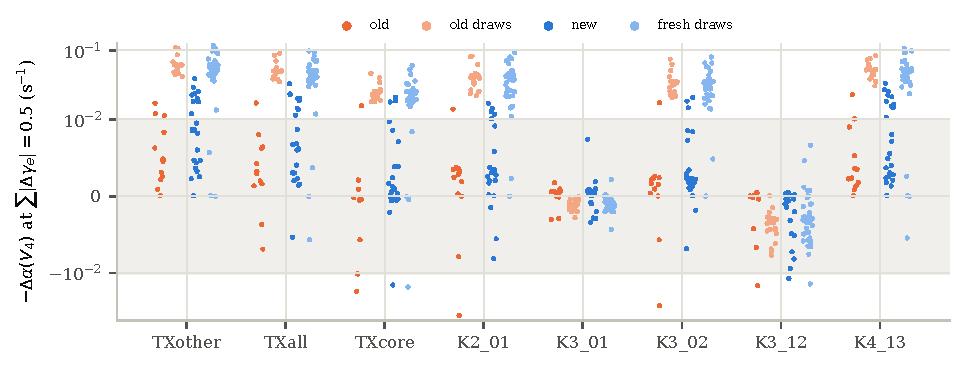
\includegraphics[width=\textwidth]{CDWH_S1_corridors.pdf}\caption{Equal-budget corridor effects by set.}\end{figure}
\begin{figure}[!h]\centering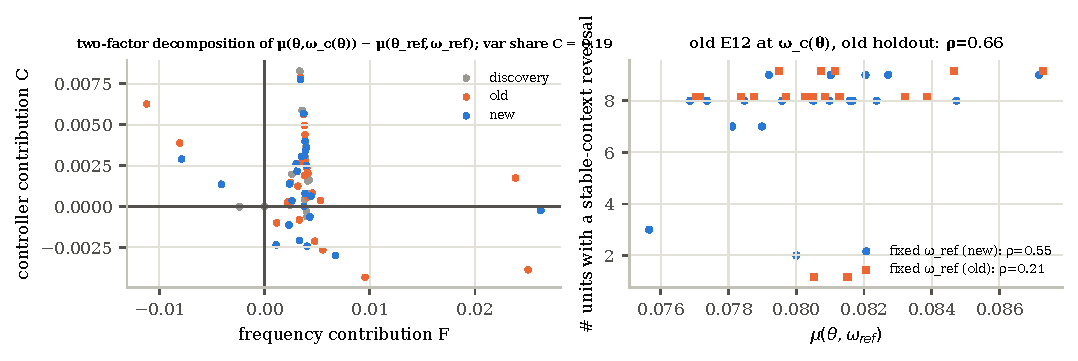
\includegraphics[width=\textwidth]{CDWH_S3_mixing.pdf}\caption{Two-factor modal-mixing decomposition and fixed-frequency correlation.}\end{figure}
\begin{figure}[!h]\centering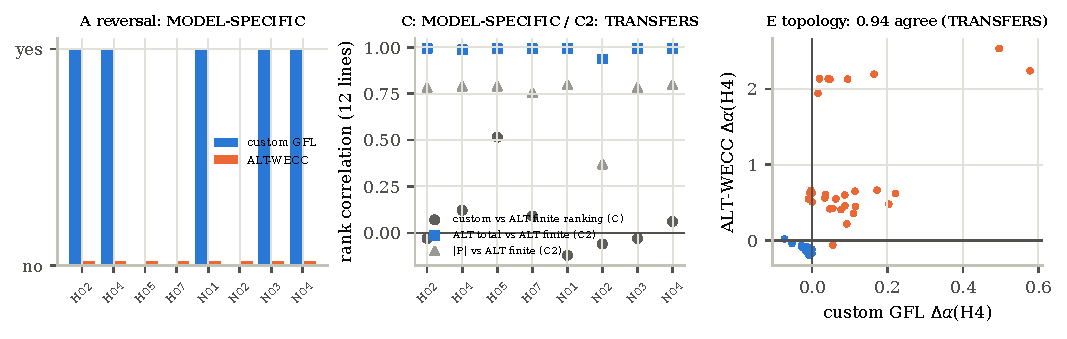
\includegraphics[width=\textwidth]{CDWH_S4_crossmodel.pdf}\caption{Cross-model holdout (ALT-WECC).}\end{figure}
\begin{figure}[!h]\centering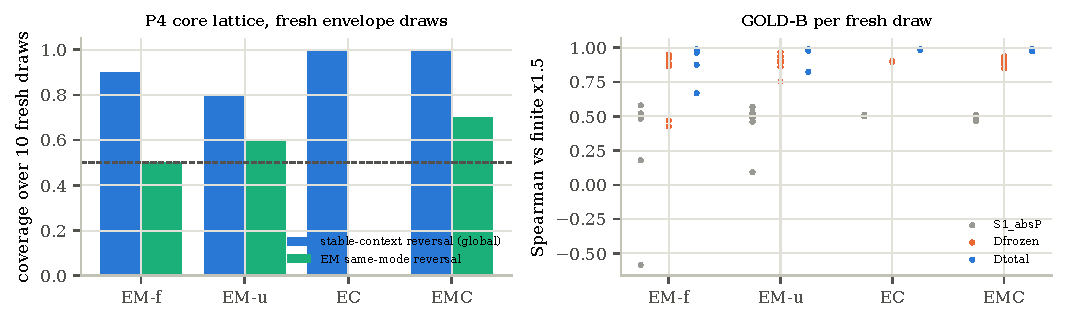
\includegraphics[width=\textwidth]{CDWH_S5_uncertainty.pdf}\caption{Fresh envelope draws: reversal coverage and branch ranking.}\end{figure}
\begin{figure}[!h]\centering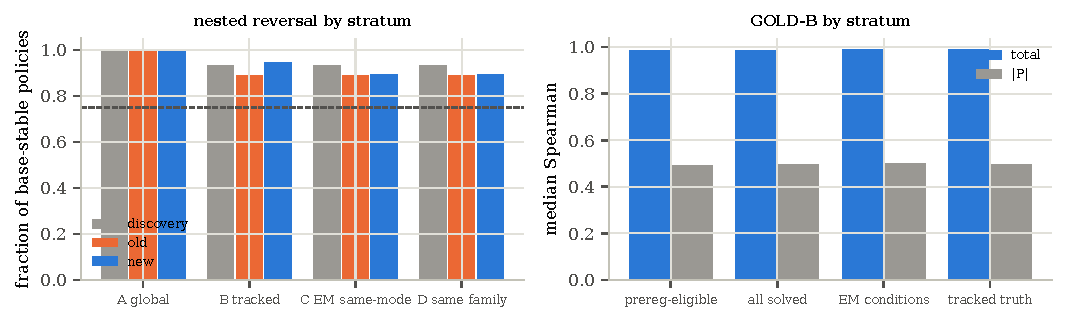
\includegraphics[width=\textwidth]{CDWH_S6_stratification.pdf}\caption{FULL / EM / same-mode stratification.}\end{figure}
\begin{figure}[!h]\centering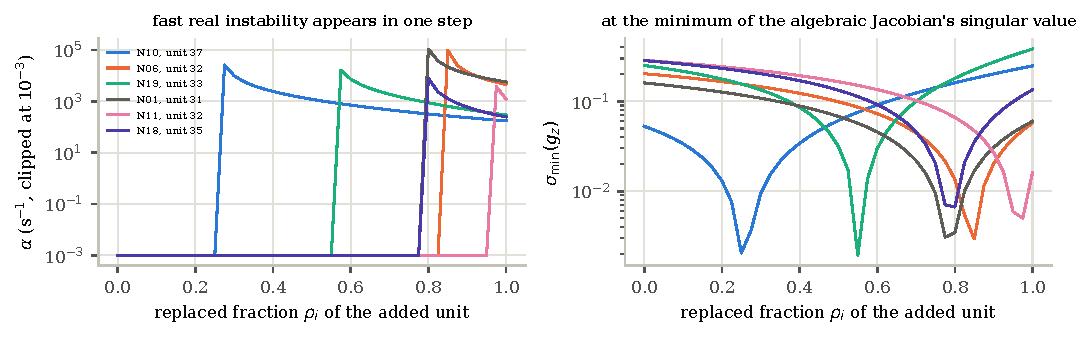
\includegraphics[width=\textwidth]{CDWH_S7_singularity.pdf}\caption{Fractional-replacement sweeps: $\aperp$ and the minimum singular value of $g_z$ against the replaced fraction.}\end{figure}
\end{document}
